\chapter{Numerical Experiments}
\label{sec:experiments}

\section{Impact of the UV Background}
The original objective of this project included a study of the dominant physical sources of Ly$\alpha$ emission, which we assumed would be stars, cooling from accreting gas, and the cosmological UV background.
As as apparent from the structure of this dissertation, the structure of the project has shifted since then, most notably to consider the underlying physical origin of Ly$\alpha$ as opposed to the astrophysical origins.
But in the case of the UV background we have an explicit simulation of this, in the ionizing radiative transfer code that we use to compute the ionization state we can adjust the intensity of the UV background that is simulated.
Elsewhere in this work we use our best estimate of a physical value for intensity of this radiation, but since it is an input to the model we can adjust it.
Ideally, we would ask some question along the lines of "What is the impact of the UV background on the formation of Ly$\alpha$ blobs?" and could answer this question by turning off the UV background and observing an impact on the Ly$\alpha$ luminosity and escape fraction.
However, we cannot address this question in such a direct manner because the impact of this phenomenon is imprinted on the temperature of the gas during the hydrodynamical simulations we rely on as inputs.

Instead, in this section we present an experiment wherein we increase the intensity of our post-processing non-heating treatment of the UV background to gain some intuition for the impact of this phenomenon on the formation of Ly$\alpha$ blobs.
We increase the intensity of the UV background from a best-guess value in \citet{Faucher-Giguere2009} up to a non-physical increase of 5 orders of magnitude (Figures~\ref{fig:big_uv_000} and \ref{fig:big_uv_005}), and find that this provides only a small enhanement to the luminosity of the blob and if anything makes it less like a blob by decreasing its spatial extent.
Our interpretation of this slight increase in luminosity and decrease in spatial extent is that the primary effect of the UV background increase is to ionize extended neutral gas which resonantly scatters the Ly$\alpha$ to greater spatial extents, permitting Ly$\alpha$ to escape the blob with less scattering.
Therefore we rule out the UV background as a driver of LAB formation and declare enhancements in the UV background uninteresting, since we increase it to a nonphysical value and still only see a marginal effect (recall that we cannot really remove the UV background because the heating it causes is accounted for in the gas temperature).


\begin{figure*}
    \centering
    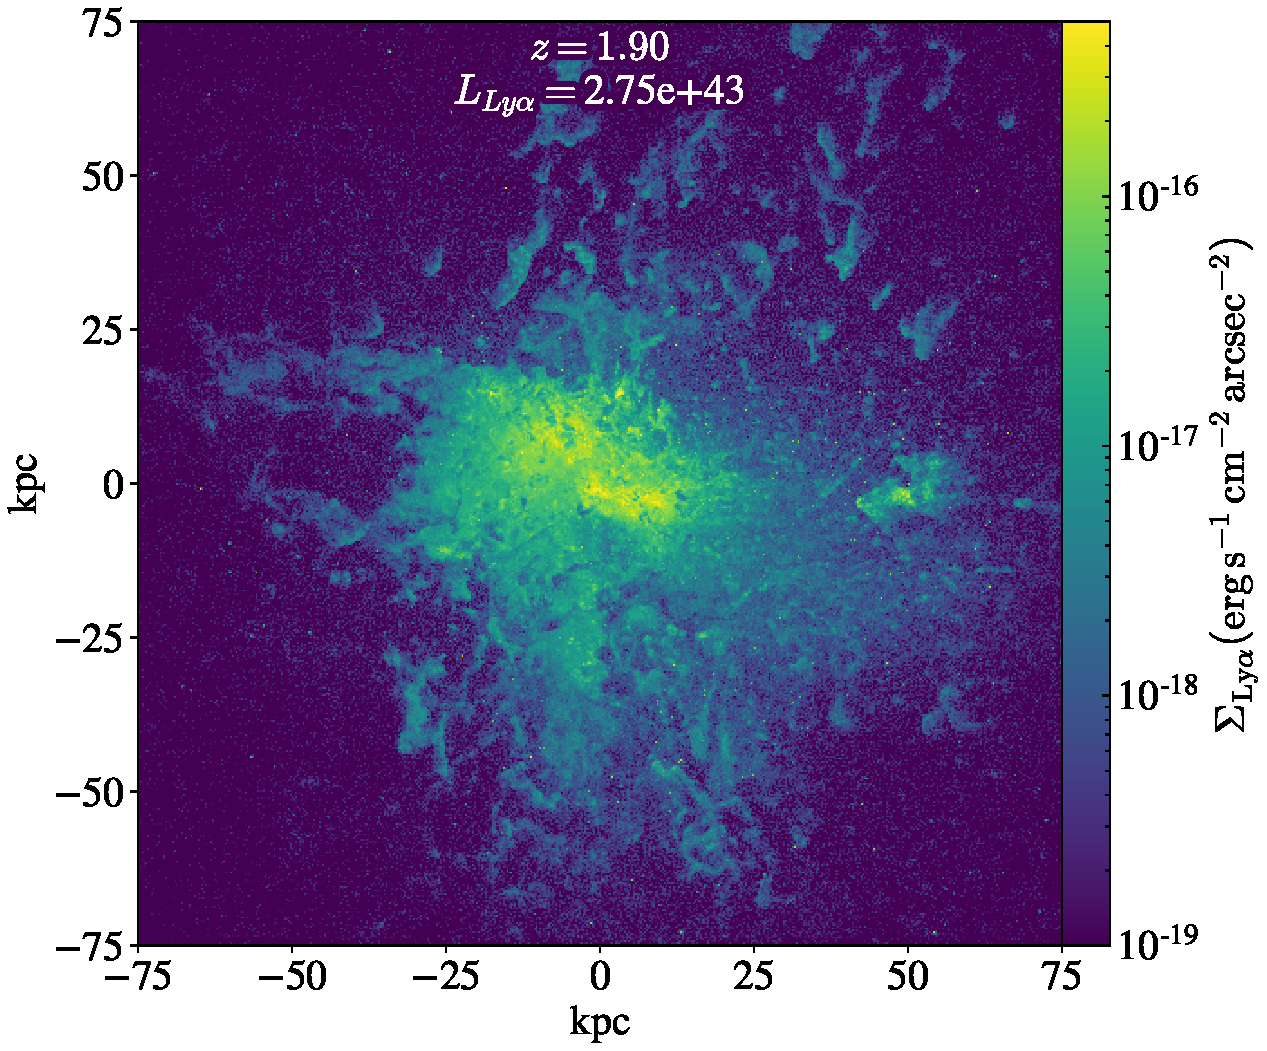
\includegraphics[width=\textwidth,keepaspectratio]{figures/big_uvb_000.pdf}
    \caption{
        A surface brightness image of a sample halo, with our best-guess UV background from \citet{Faucher-Giguere2009}.
    }
  \label{fig:big_uv_000}
\end{figure*}

\begin{figure*}
    \centering
    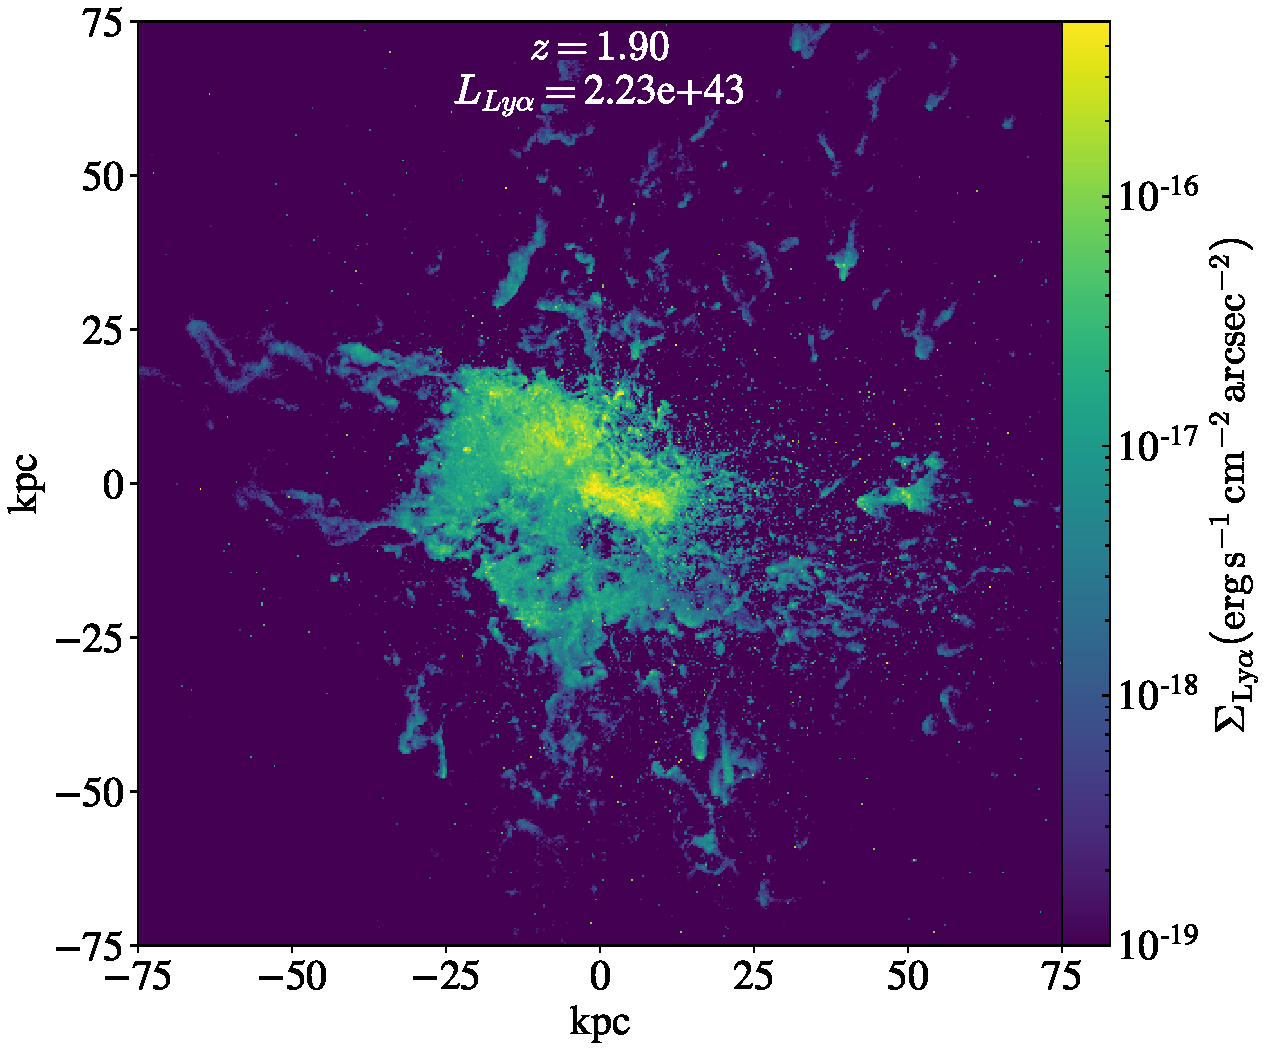
\includegraphics[width=\textwidth,keepaspectratio]{figures/big_uvb_005.pdf}
    \caption{
        A surface brightness image of a sample halo, with a UV background intensity set to $10^{5}$ times that in Figure~\ref{fig:big_uv_000}.
    }
  \label{fig:big_uv_005}
\end{figure*}



\section{MCRT Convergence}
Sometimes radiative transfer work is referred to as simulations but we try to avoid that term in this work.
Instead, we find it much better to call all our RT codebases solvers because they do not involve a time domain, and because each execution of the program proceeds through a numerical process which proceeds towards a consistent result through a different pathway.
Ideally, we'd like to know if our simulation is converged.
But answering that question is very complex as we will discuss later, so in this section we present some preliminary work on a metric for the convergence of surface brightness images.

Ideally, we should have an on-the-fly metric that measures how uncertain a particular value in the simulation is.
Since some of our work is centered around surface brightness images, a reasonable first step is to establish a metric for determining if any given pixel is converged.
To approach this, we insert a notional error map into {\sc colt}, where the uncertainty $\sigma$ of a pixel in the map due to $i$ next event estimations $e$ is
\begin{equation}
    \sigma \propto \frac{\sqrt{\Sigma_{i} e_{i}^{2}}}{\Sigma_{i} e_{i}}
    \label{eq:sb_uncertainty}
\end{equation}
This metric is essentially the relative variance within the pixel, and from a naive perspective is an effective way to track the uncertainty.
We plot this metric for one of our surface brightness images in Figure~\ref{fig:on_the_fly}.
To check how accurate this is, we run {\sc colt} 300 times with the same inputs and plot the per-pixel variance in Figure~\ref{fig:run_to_run}, which should match with Figure~\ref{fig:on_the_fly}.
As we can see, this simple on-the-fly uncertainty estimate vastly underestimates the variation in a pixel between executions of the code.

The reason this simplistic metric is wrong is beyond the scope of this work.
Instead, our purpose here is to present these results because they cost many CPU-hours and we have verified that using a naive approach to on-the-fly assessment of MCRT convergence results in an incorrect metric.
Future work on this should instead follow methodologies used in Markov Chain Monte-Carlo (MCMC) techniques, and in particular we suggest the Gelman-Rubin diagnostic may be a much better indicator of convergence (Aaron Smith, private communication).

\begin{figure*}
    \centering
    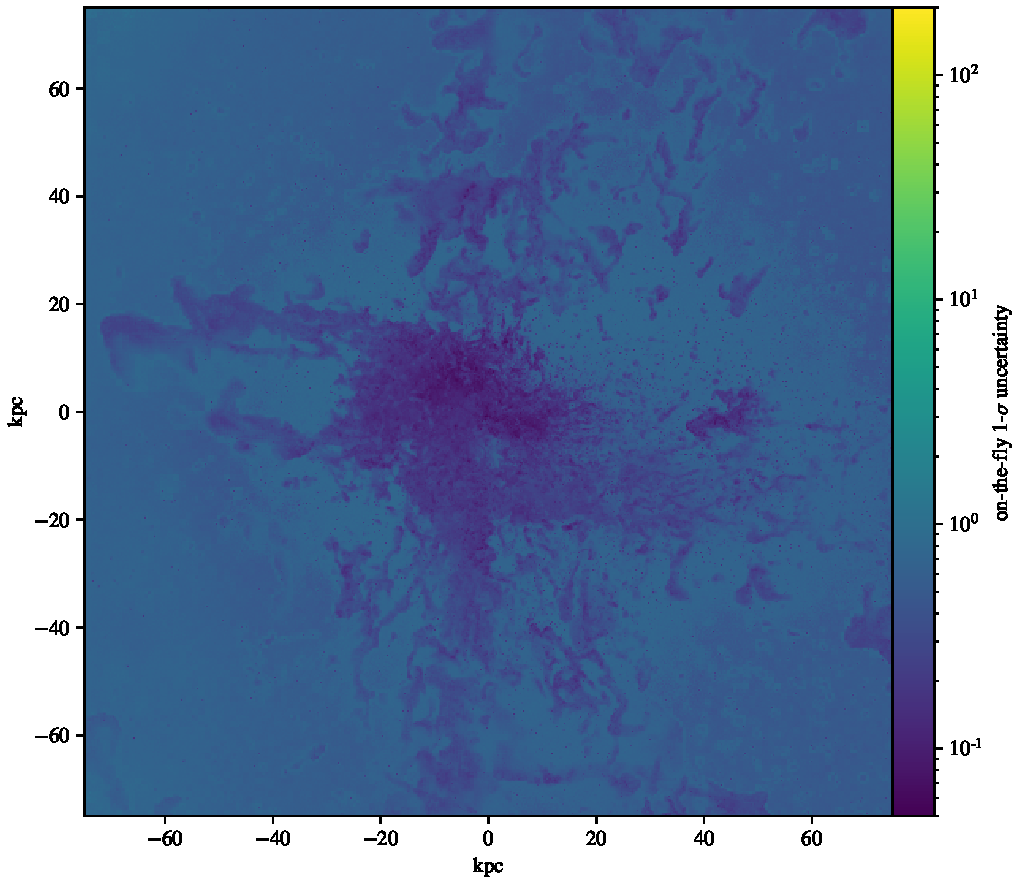
\includegraphics[width=\textwidth,keepaspectratio]{figures/on_the_fly.pdf}
    \caption{
        For a sample halo, we plot the relative uncertainty reported by Eq~\ref{eq:sb_uncertainty}.
    }
  \label{fig:on_the_fly}
\end{figure*}

\begin{figure*}
    \centering
    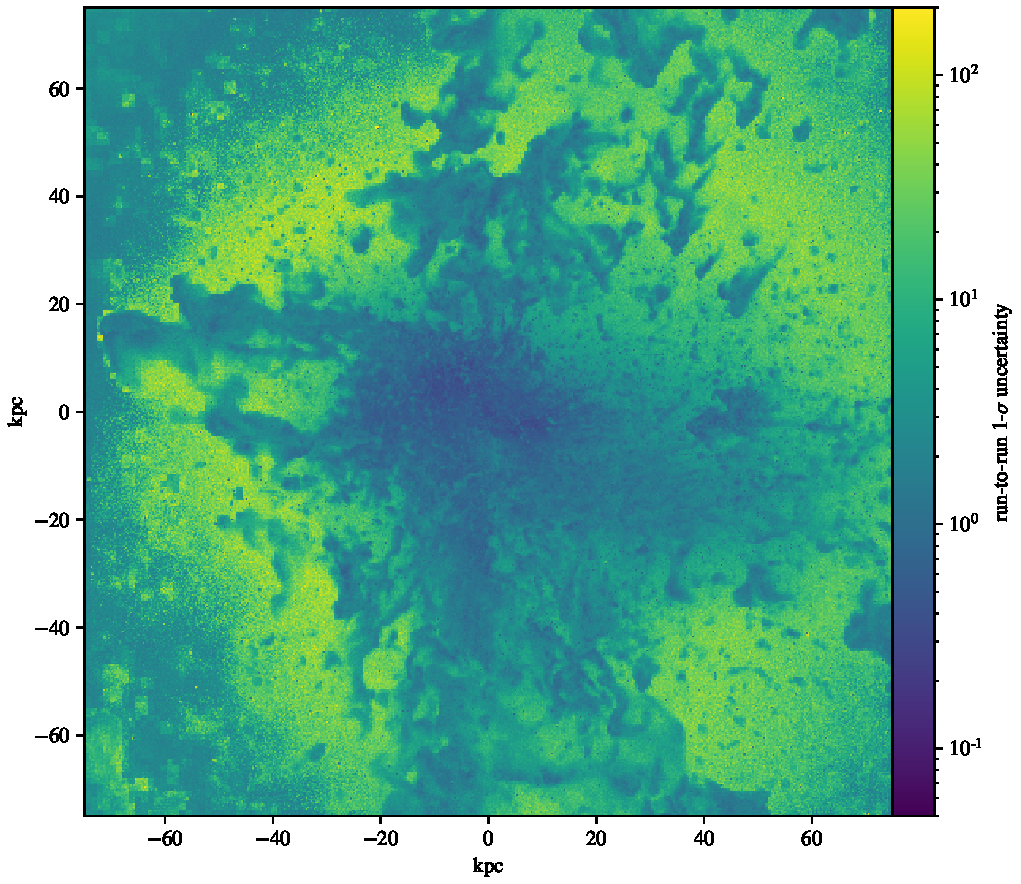
\includegraphics[width=\textwidth,keepaspectratio]{figures/run_to_run.pdf}
    \caption{
        For a sample halo, we plot the relative 1-$\sigma$ uncertainty computed across 300 runs of {\sc colt}.
        Note that this uncertainty is much greater than what is estimatedin Figure~\ref{fig:on_the_fly}.
    }
  \label{fig:run_to_run}
\end{figure*}


\section{Ionization State Extremes}
\label{sec:ionization_extremes}
In this work we have made somewhat of a big deal out of the ionization state of the gas because it is related to Ly$\alpha$ luminsity, escape fraction, and also determines which of the two physical mechanisms (recombination and collisional excitation) dominates.
For most of our work we endeavor to recreate the physical conditions that exist in nature, but of course we can write a little bit of code and adjust the physical conditions in a simulation to whatever we desire.

In this section we use this ability to get some handle on how bright a blob could be due to recombinations or collisional excitations if the ioniation state of the gas were tuned such that those mechanisms were as dominant as possible.
In the case of recombinations, we consider a scenario where all gas in the simulation is fully ionized.
This is nonphysical because there is dense cool gas in the simulation which would rapidly recombine then stay recombined if this were the case, but of course we need not let that stop us.
We present the results of this experiment in Figure~\ref{fig:rogues_fully_ionized}.
These images can be compared to Figure~\ref{fig:rogues4}, with the caution that a number of pixels that have increased in brightness are clipped in these surface brightness images produced with the altered ionization state.
We prefer this visualization to one where we have altered the scaling because it is easier to compare to the physically motivated model.
In these images, the blob appears to have shrunk even though we have altered the ionization state of the gas such that overall it enhances the luminosity of the blob.
This size decrease should not be too surprising; by ionizing the gas we have removed resonant scattering from the model so what is left is nearly a projection of Ly$\alpha$ surface luminosity (but with Monte-Carlo noise and some dust scattering).
Additionally, the luminosity in this case is enhanced by about 2 orders of magnitude; these halos have a luminosity of about $5\times10^{45}\ \rm{erg}\ \rm{s}^{-1}$

\begin{figure*}
    \centering
    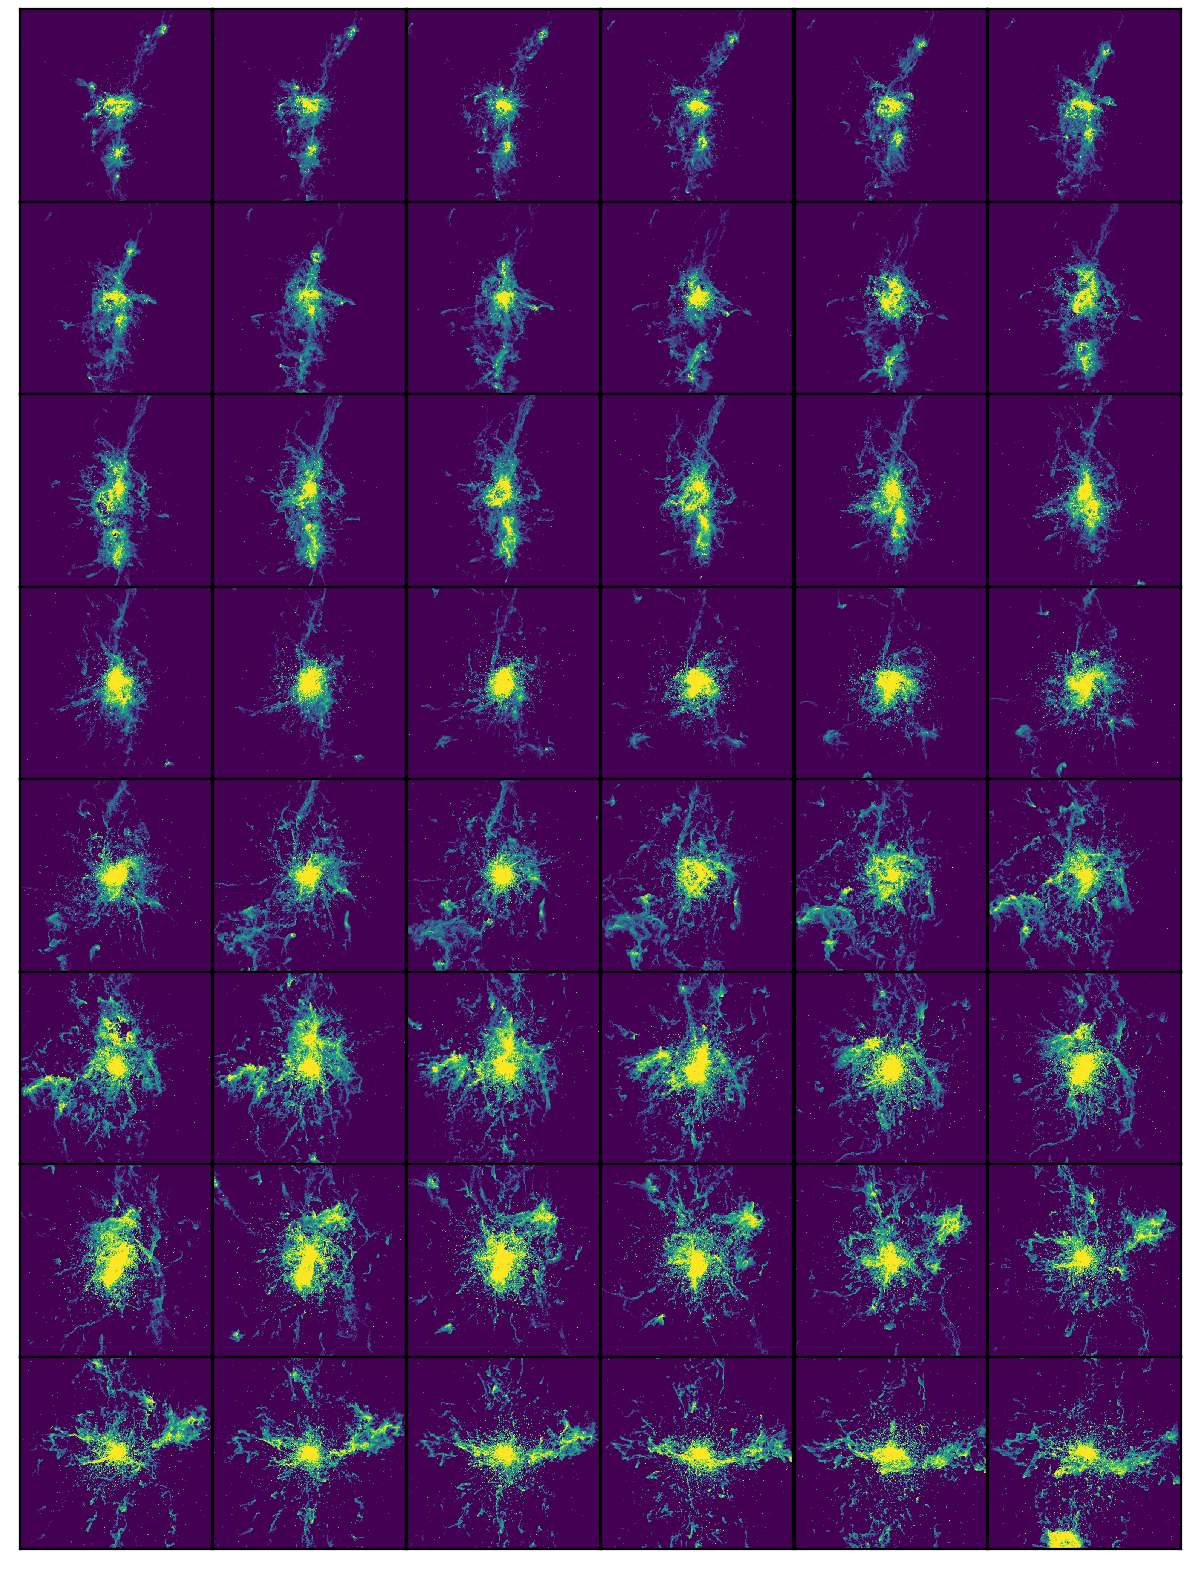
\includegraphics[width=\textwidth,keepaspectratio]{figures/rogues_fully_ionized.png}
    \caption{
        Ly$\alpha$ surface brightness images of of halo A4 from $z=4.5$ (top-left) to $z=2.0$ (bottom-right).
        All images are 75$\times$75 physical kpc across, and are scaled from $2\times10^{-19}-10^{-16}\ \rm{erg}\ \rm{s}^{-1}\ \rm{cm}^{-2}\ \rm{arcsec}^{-2}$.
    }
  \label{fig:rogues_fully_ionized}
\end{figure*}


We also conduct another experiment in which we set the ionization state of all the gas to $0.5$, to maximize the emission due to collisional excitation.
The results of this experiment are presented in Figure~\ref{fig:rogues_half_ionized}.
In this experiment we must rescaled the surface brightness images to accomodate the increased luminosity of the gas, otherwise the entire surface brightness images would be clipped.
Additionally, the luminosity in this case is enhanced by about 3 orders of magnitude; these halos have a luminosity of about $2\times10^{46}\ \rm{erg}\ \rm{s}^{-1}$.
Naively one might expext these simulations to have a much lower escape fraction since we have taken a large amount of halo gas which was previously fully ionized and put in an ionization state where it is more likely to keep Ly$\alpha$ trapped.
This is not the case; overall we see escape fractions which are approximately the same as the physically motivated case.
Most likely, this is driven by the increased emission in the hot gas which can easily escape the simulation compensating for the increased absorption of gas emitted in the more dense regions of the simulation.

\begin{figure*}
    \centering
    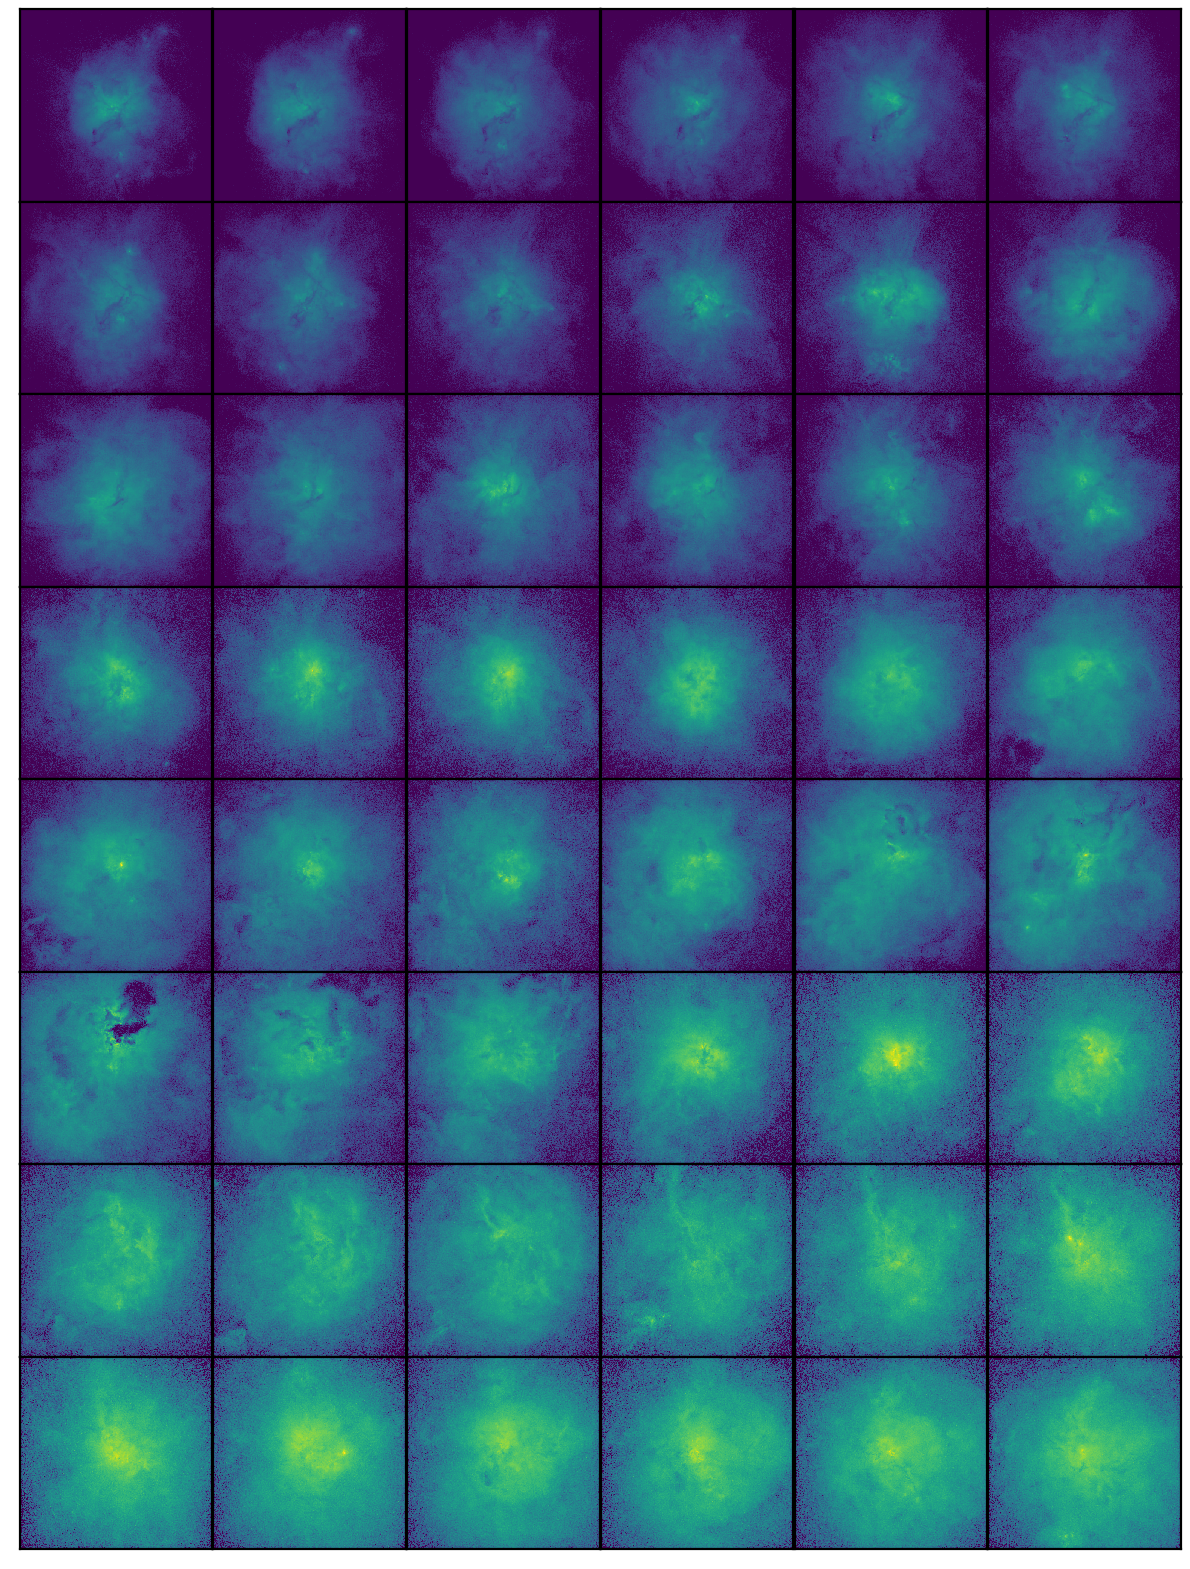
\includegraphics[width=\textwidth,keepaspectratio]{figures/rogues_half_ionized.png}
    \caption{
        Ly$\alpha$ surface brightness images of of halo A4 from $z=4.5$ (top-left) to $z=2.0$ (bottom-right), where we have artificially set the ionization state to $0.5$.
        All images are 75$\times$75 physical kpc across, and are scaled from $1\times10^{-13}-10^{-17}\ \rm{erg}\ \rm{s}^{-1}\ \rm{cm}^{-2}\ \rm{arcsec}^{-2}$.
    }
  \label{fig:rogues_half_ionized}
\end{figure*}


